% Graphe de dependances des concepts - LearnByAoc
% A inclure dans le document principal avec % Graphe de dependances des concepts - LearnByAoc
% A inclure dans le document principal avec % Graphe de dependances des concepts - LearnByAoc
% A inclure dans le document principal avec % Graphe de dependances des concepts - LearnByAoc
% A inclure dans le document principal avec \input{assets/dependency_graph.tex}

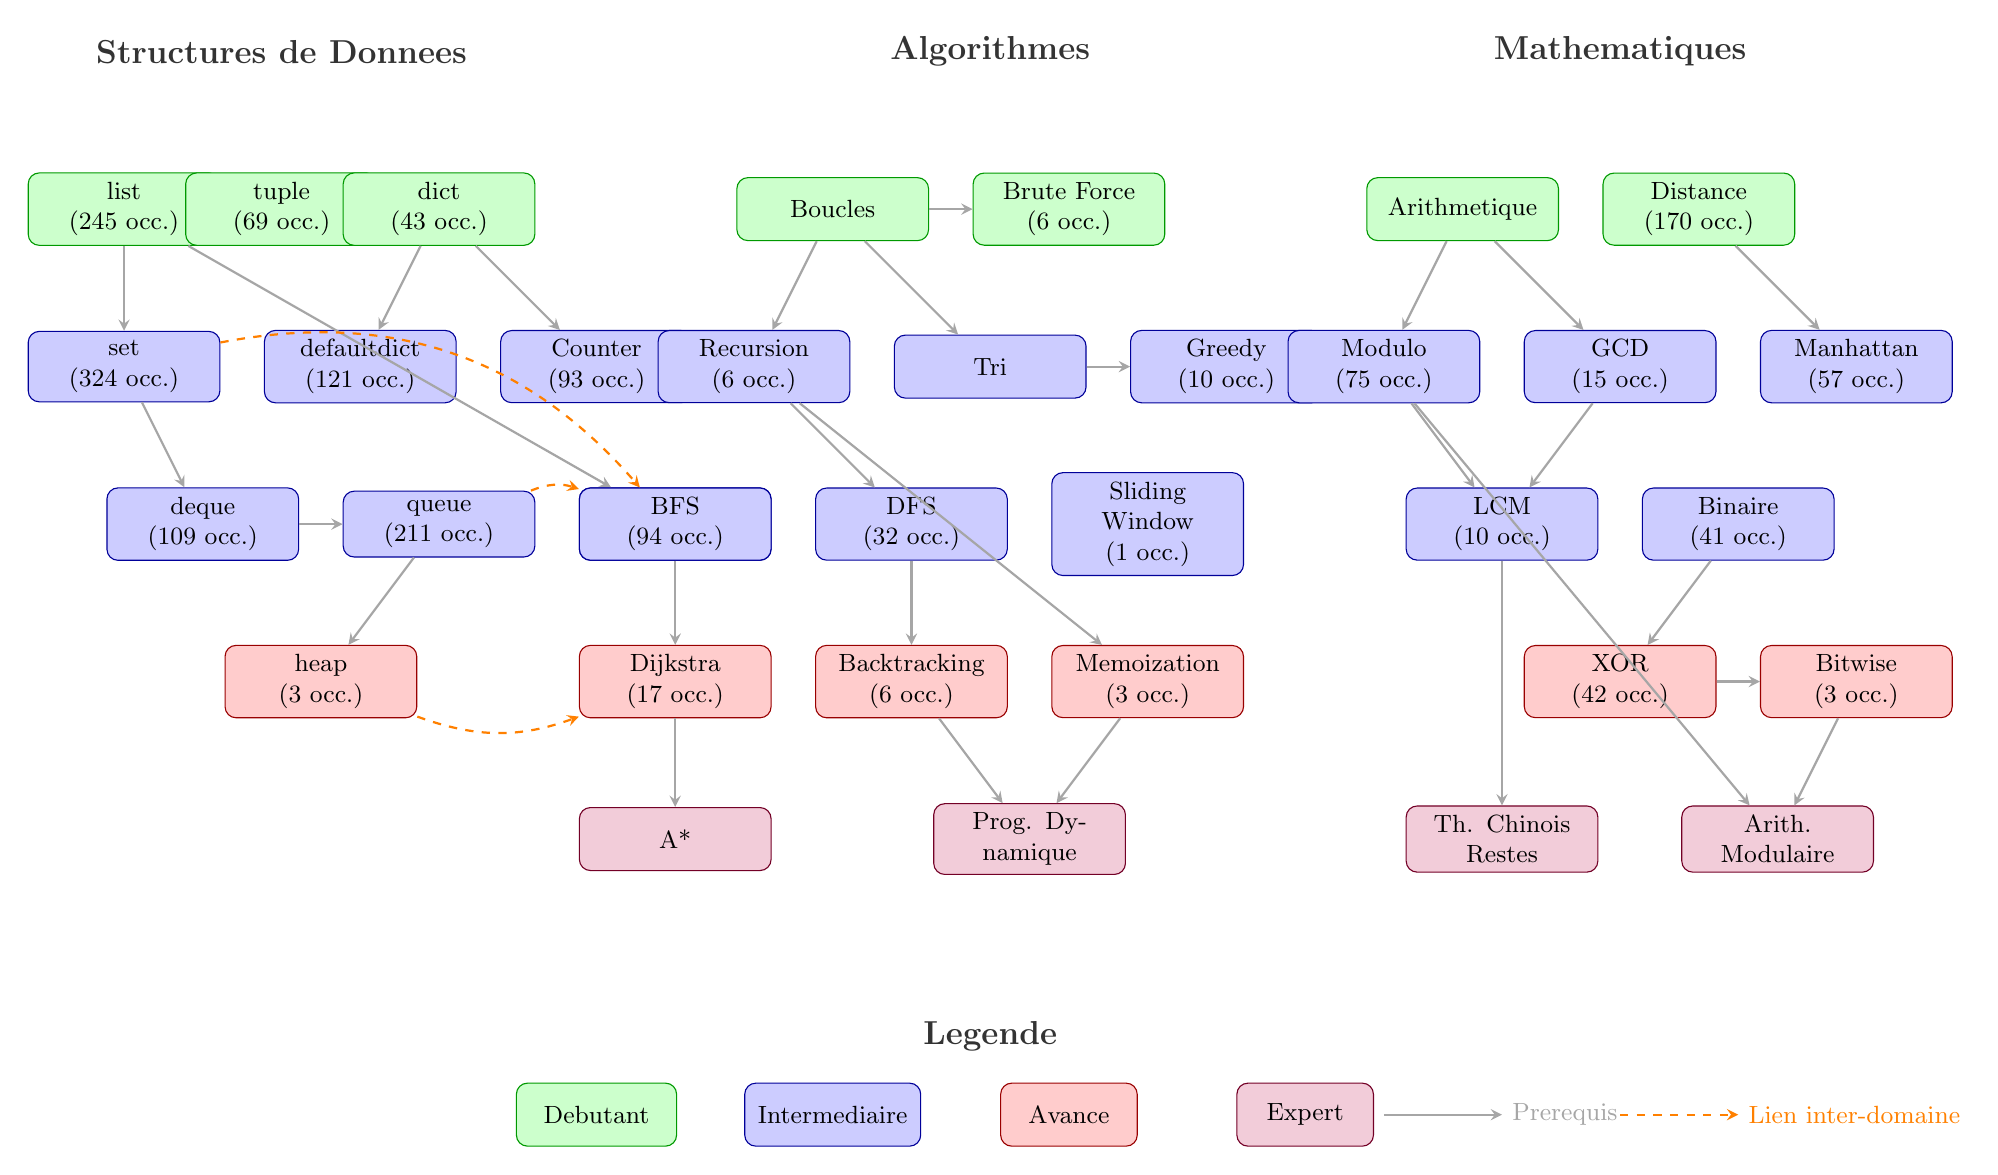
\begin{tikzpicture}[
    % Styles des noeuds par niveau
    debutant/.style={rectangle, rounded corners, draw=green!60!black, fill=green!20,
                     text width=2.2cm, align=center, minimum height=0.8cm, font=\small},
    intermediaire/.style={rectangle, rounded corners, draw=blue!60!black, fill=blue!20,
                          text width=2.2cm, align=center, minimum height=0.8cm, font=\small},
    avance/.style={rectangle, rounded corners, draw=red!60!black, fill=red!20,
                   text width=2.2cm, align=center, minimum height=0.8cm, font=\small},
    expert/.style={rectangle, rounded corners, draw=purple!60!black, fill=purple!20,
                   text width=2.2cm, align=center, minimum height=0.8cm, font=\small},
    % Style des fleches
    arrow/.style={->, >=stealth, thick, color=gray!70},
    % Style des labels de section
    section/.style={font=\bfseries\large, color=black!80}
]

% ==========================================
% SECTION 1: STRUCTURES DE DONNEES (gauche)
% ==========================================
\node[section] at (-6, 8) {Structures de Donnees};

% Niveau Debutant
\node[debutant] (list) at (-8, 6) {list\\(245 occ.)};
\node[debutant] (tuple) at (-6, 6) {tuple\\(69 occ.)};
\node[debutant] (dict) at (-4, 6) {dict\\(43 occ.)};

% Niveau Intermediaire
\node[intermediaire] (set) at (-8, 4) {set\\(324 occ.)};
\node[intermediaire] (defaultdict) at (-5, 4) {defaultdict\\(121 occ.)};
\node[intermediaire] (counter) at (-2, 4) {Counter\\(93 occ.)};

% Niveau Intermediaire+
\node[intermediaire] (deque) at (-7, 2) {deque\\(109 occ.)};
\node[intermediaire] (queue) at (-4, 2) {queue\\(211 occ.)};
\node[intermediaire] (stack) at (-1, 2) {stack\\(98 occ.)};

% Niveau Avance
\node[avance] (heap) at (-5.5, 0) {heap\\(3 occ.)};

% Fleches structures
\draw[arrow] (list) -- (set);
\draw[arrow] (dict) -- (defaultdict);
\draw[arrow] (dict) -- (counter);
\draw[arrow] (set) -- (deque);
\draw[arrow] (deque) -- (queue);
\draw[arrow] (list) -- (stack);
\draw[arrow] (queue) -- (heap);

% ==========================================
% SECTION 2: ALGORITHMES (centre)
% ==========================================
\node[section] at (3, 8) {Algorithmes};

% Niveau Debutant
\node[debutant] (boucles) at (1, 6) {Boucles};
\node[debutant] (brute) at (4, 6) {Brute Force\\(6 occ.)};

% Niveau Intermediaire
\node[intermediaire] (recursion) at (0, 4) {Recursion\\(6 occ.)};
\node[intermediaire] (tri) at (3, 4) {Tri};
\node[intermediaire] (greedy) at (6, 4) {Greedy\\(10 occ.)};

% Niveau Intermediaire+
\node[intermediaire] (bfs) at (-1, 2) {BFS\\(94 occ.)};
\node[intermediaire] (dfs) at (2, 2) {DFS\\(32 occ.)};
\node[intermediaire] (sliding) at (5, 2) {Sliding Window\\(1 occ.)};

% Niveau Avance
\node[avance] (dijkstra) at (-1, 0) {Dijkstra\\(17 occ.)};
\node[avance] (backtrack) at (2, 0) {Backtracking\\(6 occ.)};
\node[avance] (memo) at (5, 0) {Memoization\\(3 occ.)};

% Niveau Expert
\node[expert] (astar) at (-1, -2) {A*};
\node[expert] (dp) at (3.5, -2) {Prog. Dynamique};

% Fleches algorithmes
\draw[arrow] (boucles) -- (brute);
\draw[arrow] (boucles) -- (recursion);
\draw[arrow] (boucles) -- (tri);
\draw[arrow] (tri) -- (greedy);
\draw[arrow] (recursion) -- (dfs);
\draw[arrow] (recursion) -- (memo);
\draw[arrow] (dfs) -- (backtrack);
\draw[arrow] (memo) -- (dp);
\draw[arrow] (backtrack) -- (dp);

% Connexions inter-sections
\draw[arrow, dashed, color=orange] (queue) to[bend left=20] (bfs);
\draw[arrow, dashed, color=orange] (set) to[bend left=30] (bfs);
\draw[arrow] (bfs) -- (dijkstra);
\draw[arrow, dashed, color=orange] (heap) to[bend right=20] (dijkstra);
\draw[arrow] (dijkstra) -- (astar);

% ==========================================
% SECTION 3: MATHEMATIQUES (droite)
% ==========================================
\node[section] at (11, 8) {Mathematiques};

% Niveau Debutant
\node[debutant] (arith) at (9, 6) {Arithmetique};
\node[debutant] (distance) at (12, 6) {Distance\\(170 occ.)};

% Niveau Intermediaire
\node[intermediaire] (modulo) at (8, 4) {Modulo\\(75 occ.)};
\node[intermediaire] (gcd) at (11, 4) {GCD\\(15 occ.)};
\node[intermediaire] (manhattan) at (14, 4) {Manhattan\\(57 occ.)};

% Niveau Intermediaire+
\node[intermediaire] (lcm) at (9.5, 2) {LCM\\(10 occ.)};
\node[intermediaire] (binary) at (12.5, 2) {Binaire\\(41 occ.)};

% Niveau Avance
\node[avance] (xor) at (11, 0) {XOR\\(42 occ.)};
\node[avance] (bitwise) at (14, 0) {Bitwise\\(3 occ.)};

% Niveau Expert
\node[expert] (crt) at (9.5, -2) {Th. Chinois\\Restes};
\node[expert] (modular) at (13, -2) {Arith.\\Modulaire};

% Fleches maths
\draw[arrow] (arith) -- (modulo);
\draw[arrow] (arith) -- (gcd);
\draw[arrow] (distance) -- (manhattan);
\draw[arrow] (gcd) -- (lcm);
\draw[arrow] (modulo) -- (lcm);
\draw[arrow] (binary) -- (xor);
\draw[arrow] (xor) -- (bitwise);
\draw[arrow] (lcm) -- (crt);
\draw[arrow] (modulo) -- (modular);
\draw[arrow] (bitwise) -- (modular);

% ==========================================
% LEGENDE
% ==========================================
\node[section] at (3, -4.5) {Legende};
\node[debutant, text width=1.8cm] at (-2, -5.5) {Debutant};
\node[intermediaire, text width=2cm] at (1, -5.5) {Intermediaire};
\node[avance, text width=1.5cm] at (4, -5.5) {Avance};
\node[expert, text width=1.5cm] at (7, -5.5) {Expert};

\draw[arrow] (8, -5.5) -- (9.5, -5.5) node[right, font=\small] {Prerequis};
\draw[arrow, dashed, color=orange] (11, -5.5) -- (12.5, -5.5) node[right, font=\small] {Lien inter-domaine};

\end{tikzpicture}


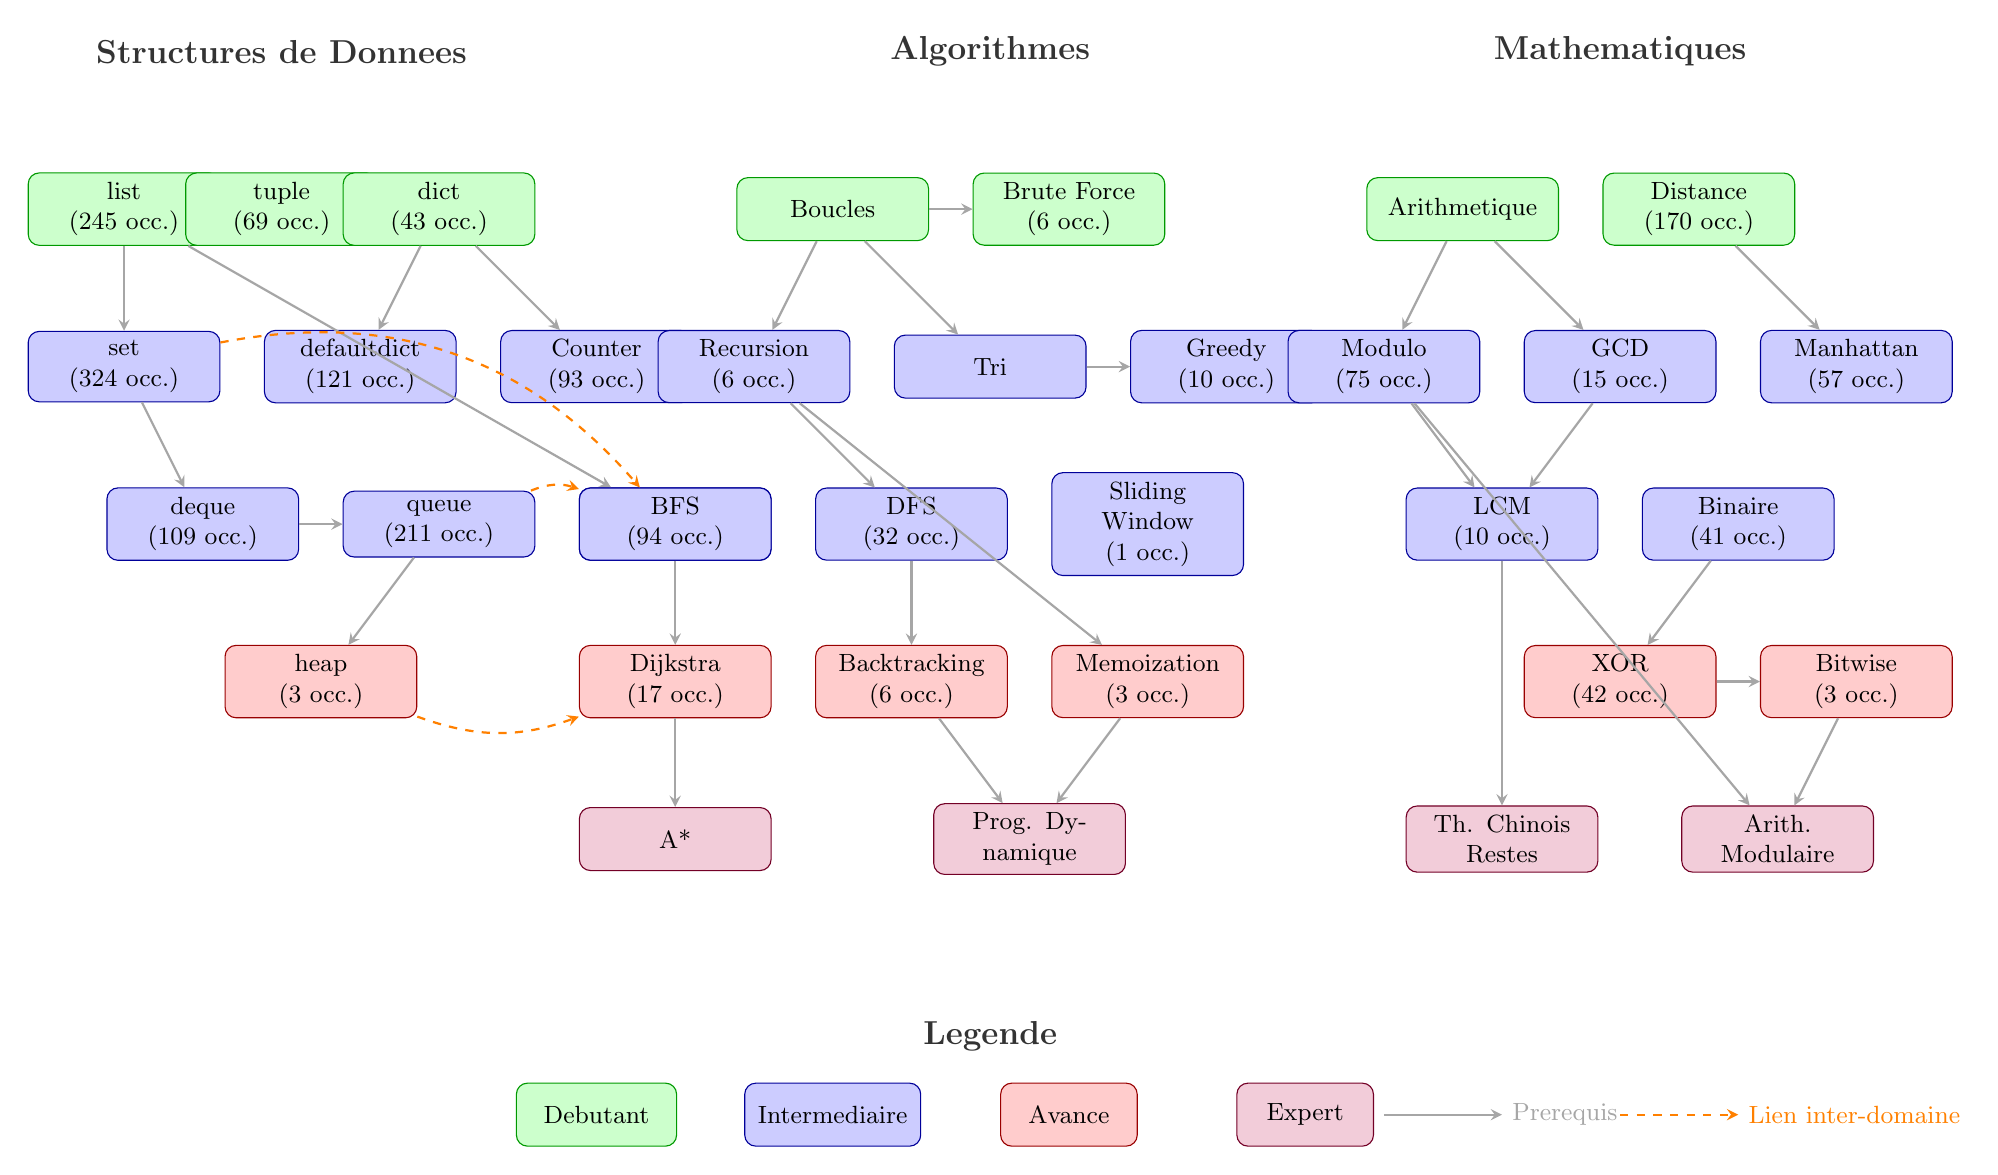
\begin{tikzpicture}[
    % Styles des noeuds par niveau
    debutant/.style={rectangle, rounded corners, draw=green!60!black, fill=green!20,
                     text width=2.2cm, align=center, minimum height=0.8cm, font=\small},
    intermediaire/.style={rectangle, rounded corners, draw=blue!60!black, fill=blue!20,
                          text width=2.2cm, align=center, minimum height=0.8cm, font=\small},
    avance/.style={rectangle, rounded corners, draw=red!60!black, fill=red!20,
                   text width=2.2cm, align=center, minimum height=0.8cm, font=\small},
    expert/.style={rectangle, rounded corners, draw=purple!60!black, fill=purple!20,
                   text width=2.2cm, align=center, minimum height=0.8cm, font=\small},
    % Style des fleches
    arrow/.style={->, >=stealth, thick, color=gray!70},
    % Style des labels de section
    section/.style={font=\bfseries\large, color=black!80}
]

% ==========================================
% SECTION 1: STRUCTURES DE DONNEES (gauche)
% ==========================================
\node[section] at (-6, 8) {Structures de Donnees};

% Niveau Debutant
\node[debutant] (list) at (-8, 6) {list\\(245 occ.)};
\node[debutant] (tuple) at (-6, 6) {tuple\\(69 occ.)};
\node[debutant] (dict) at (-4, 6) {dict\\(43 occ.)};

% Niveau Intermediaire
\node[intermediaire] (set) at (-8, 4) {set\\(324 occ.)};
\node[intermediaire] (defaultdict) at (-5, 4) {defaultdict\\(121 occ.)};
\node[intermediaire] (counter) at (-2, 4) {Counter\\(93 occ.)};

% Niveau Intermediaire+
\node[intermediaire] (deque) at (-7, 2) {deque\\(109 occ.)};
\node[intermediaire] (queue) at (-4, 2) {queue\\(211 occ.)};
\node[intermediaire] (stack) at (-1, 2) {stack\\(98 occ.)};

% Niveau Avance
\node[avance] (heap) at (-5.5, 0) {heap\\(3 occ.)};

% Fleches structures
\draw[arrow] (list) -- (set);
\draw[arrow] (dict) -- (defaultdict);
\draw[arrow] (dict) -- (counter);
\draw[arrow] (set) -- (deque);
\draw[arrow] (deque) -- (queue);
\draw[arrow] (list) -- (stack);
\draw[arrow] (queue) -- (heap);

% ==========================================
% SECTION 2: ALGORITHMES (centre)
% ==========================================
\node[section] at (3, 8) {Algorithmes};

% Niveau Debutant
\node[debutant] (boucles) at (1, 6) {Boucles};
\node[debutant] (brute) at (4, 6) {Brute Force\\(6 occ.)};

% Niveau Intermediaire
\node[intermediaire] (recursion) at (0, 4) {Recursion\\(6 occ.)};
\node[intermediaire] (tri) at (3, 4) {Tri};
\node[intermediaire] (greedy) at (6, 4) {Greedy\\(10 occ.)};

% Niveau Intermediaire+
\node[intermediaire] (bfs) at (-1, 2) {BFS\\(94 occ.)};
\node[intermediaire] (dfs) at (2, 2) {DFS\\(32 occ.)};
\node[intermediaire] (sliding) at (5, 2) {Sliding Window\\(1 occ.)};

% Niveau Avance
\node[avance] (dijkstra) at (-1, 0) {Dijkstra\\(17 occ.)};
\node[avance] (backtrack) at (2, 0) {Backtracking\\(6 occ.)};
\node[avance] (memo) at (5, 0) {Memoization\\(3 occ.)};

% Niveau Expert
\node[expert] (astar) at (-1, -2) {A*};
\node[expert] (dp) at (3.5, -2) {Prog. Dynamique};

% Fleches algorithmes
\draw[arrow] (boucles) -- (brute);
\draw[arrow] (boucles) -- (recursion);
\draw[arrow] (boucles) -- (tri);
\draw[arrow] (tri) -- (greedy);
\draw[arrow] (recursion) -- (dfs);
\draw[arrow] (recursion) -- (memo);
\draw[arrow] (dfs) -- (backtrack);
\draw[arrow] (memo) -- (dp);
\draw[arrow] (backtrack) -- (dp);

% Connexions inter-sections
\draw[arrow, dashed, color=orange] (queue) to[bend left=20] (bfs);
\draw[arrow, dashed, color=orange] (set) to[bend left=30] (bfs);
\draw[arrow] (bfs) -- (dijkstra);
\draw[arrow, dashed, color=orange] (heap) to[bend right=20] (dijkstra);
\draw[arrow] (dijkstra) -- (astar);

% ==========================================
% SECTION 3: MATHEMATIQUES (droite)
% ==========================================
\node[section] at (11, 8) {Mathematiques};

% Niveau Debutant
\node[debutant] (arith) at (9, 6) {Arithmetique};
\node[debutant] (distance) at (12, 6) {Distance\\(170 occ.)};

% Niveau Intermediaire
\node[intermediaire] (modulo) at (8, 4) {Modulo\\(75 occ.)};
\node[intermediaire] (gcd) at (11, 4) {GCD\\(15 occ.)};
\node[intermediaire] (manhattan) at (14, 4) {Manhattan\\(57 occ.)};

% Niveau Intermediaire+
\node[intermediaire] (lcm) at (9.5, 2) {LCM\\(10 occ.)};
\node[intermediaire] (binary) at (12.5, 2) {Binaire\\(41 occ.)};

% Niveau Avance
\node[avance] (xor) at (11, 0) {XOR\\(42 occ.)};
\node[avance] (bitwise) at (14, 0) {Bitwise\\(3 occ.)};

% Niveau Expert
\node[expert] (crt) at (9.5, -2) {Th. Chinois\\Restes};
\node[expert] (modular) at (13, -2) {Arith.\\Modulaire};

% Fleches maths
\draw[arrow] (arith) -- (modulo);
\draw[arrow] (arith) -- (gcd);
\draw[arrow] (distance) -- (manhattan);
\draw[arrow] (gcd) -- (lcm);
\draw[arrow] (modulo) -- (lcm);
\draw[arrow] (binary) -- (xor);
\draw[arrow] (xor) -- (bitwise);
\draw[arrow] (lcm) -- (crt);
\draw[arrow] (modulo) -- (modular);
\draw[arrow] (bitwise) -- (modular);

% ==========================================
% LEGENDE
% ==========================================
\node[section] at (3, -4.5) {Legende};
\node[debutant, text width=1.8cm] at (-2, -5.5) {Debutant};
\node[intermediaire, text width=2cm] at (1, -5.5) {Intermediaire};
\node[avance, text width=1.5cm] at (4, -5.5) {Avance};
\node[expert, text width=1.5cm] at (7, -5.5) {Expert};

\draw[arrow] (8, -5.5) -- (9.5, -5.5) node[right, font=\small] {Prerequis};
\draw[arrow, dashed, color=orange] (11, -5.5) -- (12.5, -5.5) node[right, font=\small] {Lien inter-domaine};

\end{tikzpicture}


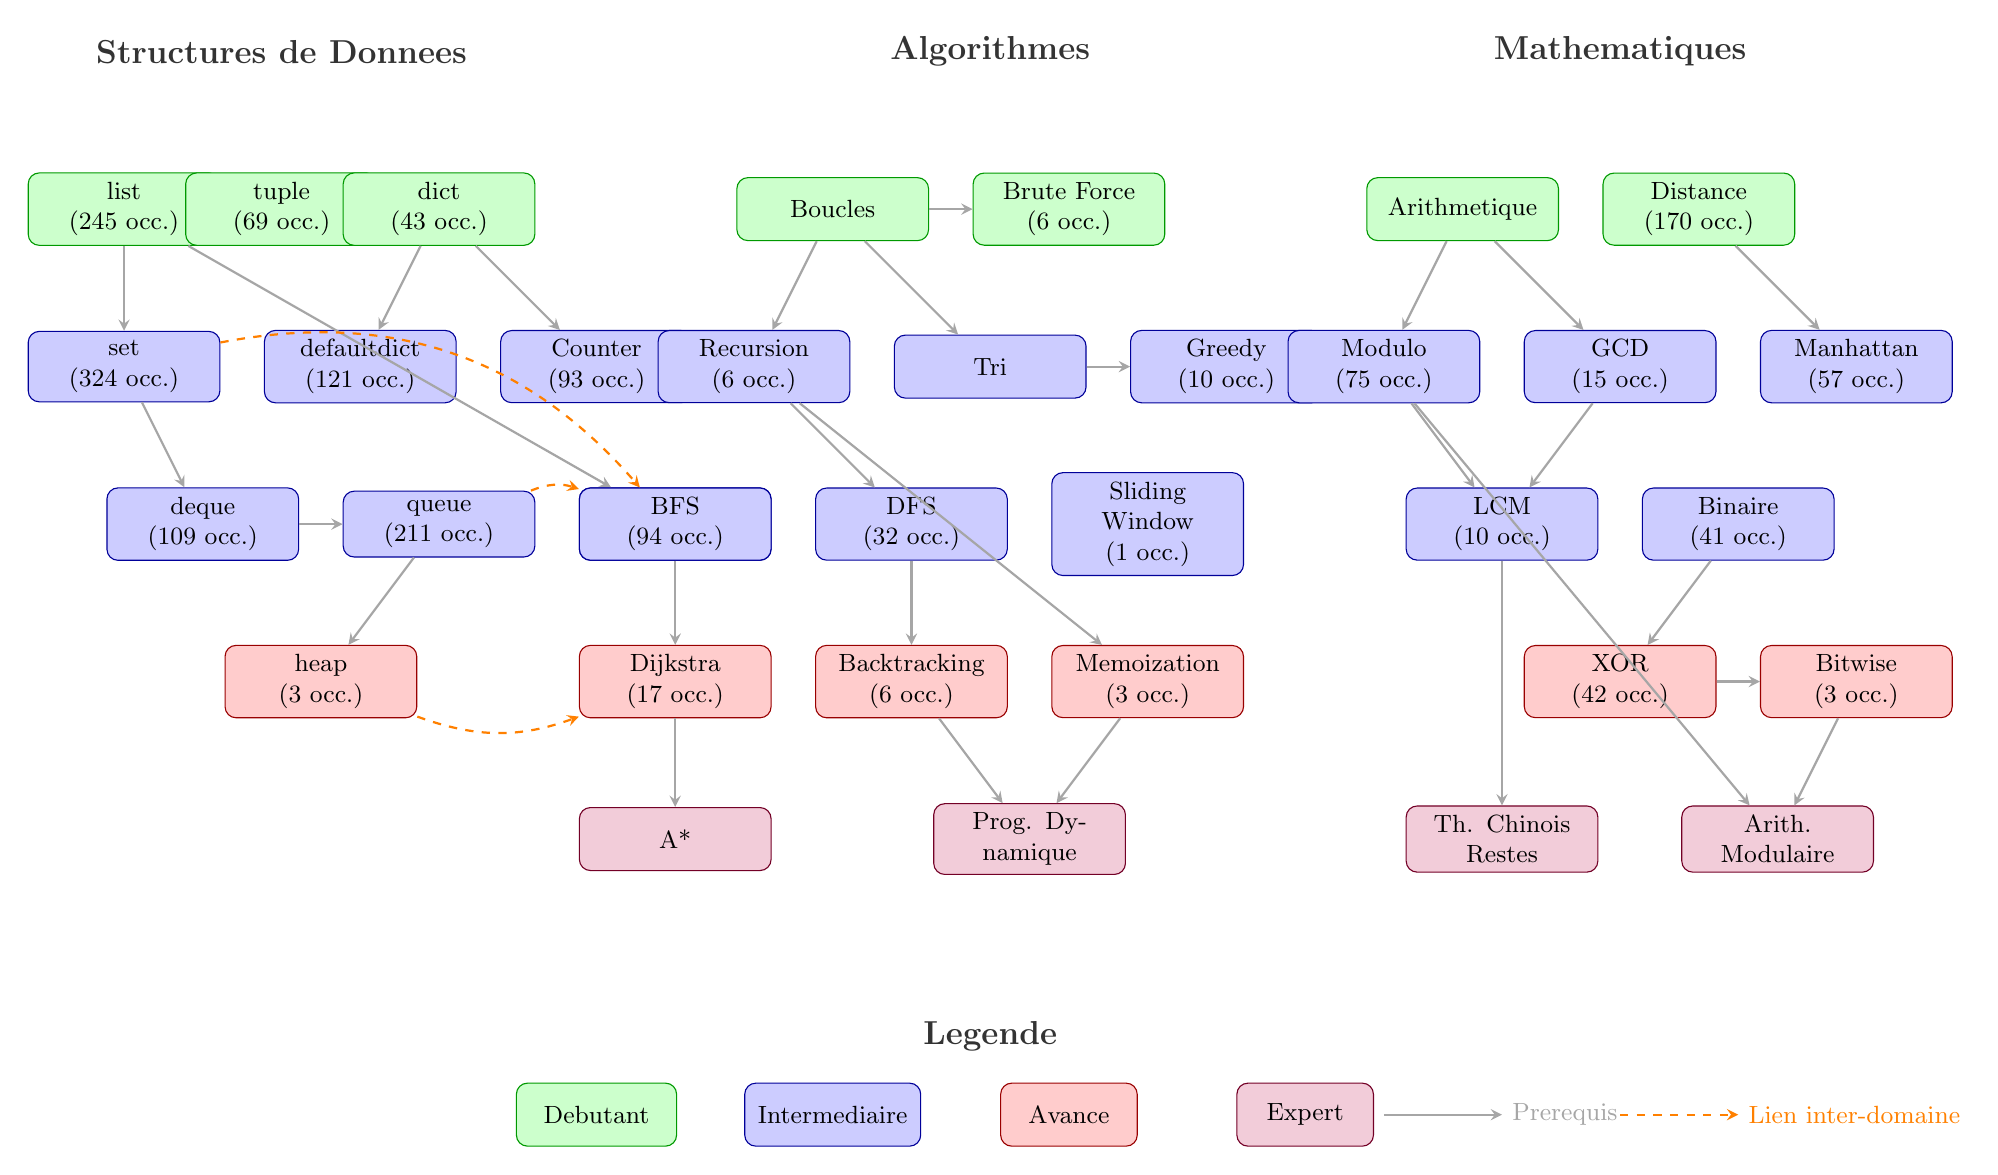
\begin{tikzpicture}[
    % Styles des noeuds par niveau
    debutant/.style={rectangle, rounded corners, draw=green!60!black, fill=green!20,
                     text width=2.2cm, align=center, minimum height=0.8cm, font=\small},
    intermediaire/.style={rectangle, rounded corners, draw=blue!60!black, fill=blue!20,
                          text width=2.2cm, align=center, minimum height=0.8cm, font=\small},
    avance/.style={rectangle, rounded corners, draw=red!60!black, fill=red!20,
                   text width=2.2cm, align=center, minimum height=0.8cm, font=\small},
    expert/.style={rectangle, rounded corners, draw=purple!60!black, fill=purple!20,
                   text width=2.2cm, align=center, minimum height=0.8cm, font=\small},
    % Style des fleches
    arrow/.style={->, >=stealth, thick, color=gray!70},
    % Style des labels de section
    section/.style={font=\bfseries\large, color=black!80}
]

% ==========================================
% SECTION 1: STRUCTURES DE DONNEES (gauche)
% ==========================================
\node[section] at (-6, 8) {Structures de Donnees};

% Niveau Debutant
\node[debutant] (list) at (-8, 6) {list\\(245 occ.)};
\node[debutant] (tuple) at (-6, 6) {tuple\\(69 occ.)};
\node[debutant] (dict) at (-4, 6) {dict\\(43 occ.)};

% Niveau Intermediaire
\node[intermediaire] (set) at (-8, 4) {set\\(324 occ.)};
\node[intermediaire] (defaultdict) at (-5, 4) {defaultdict\\(121 occ.)};
\node[intermediaire] (counter) at (-2, 4) {Counter\\(93 occ.)};

% Niveau Intermediaire+
\node[intermediaire] (deque) at (-7, 2) {deque\\(109 occ.)};
\node[intermediaire] (queue) at (-4, 2) {queue\\(211 occ.)};
\node[intermediaire] (stack) at (-1, 2) {stack\\(98 occ.)};

% Niveau Avance
\node[avance] (heap) at (-5.5, 0) {heap\\(3 occ.)};

% Fleches structures
\draw[arrow] (list) -- (set);
\draw[arrow] (dict) -- (defaultdict);
\draw[arrow] (dict) -- (counter);
\draw[arrow] (set) -- (deque);
\draw[arrow] (deque) -- (queue);
\draw[arrow] (list) -- (stack);
\draw[arrow] (queue) -- (heap);

% ==========================================
% SECTION 2: ALGORITHMES (centre)
% ==========================================
\node[section] at (3, 8) {Algorithmes};

% Niveau Debutant
\node[debutant] (boucles) at (1, 6) {Boucles};
\node[debutant] (brute) at (4, 6) {Brute Force\\(6 occ.)};

% Niveau Intermediaire
\node[intermediaire] (recursion) at (0, 4) {Recursion\\(6 occ.)};
\node[intermediaire] (tri) at (3, 4) {Tri};
\node[intermediaire] (greedy) at (6, 4) {Greedy\\(10 occ.)};

% Niveau Intermediaire+
\node[intermediaire] (bfs) at (-1, 2) {BFS\\(94 occ.)};
\node[intermediaire] (dfs) at (2, 2) {DFS\\(32 occ.)};
\node[intermediaire] (sliding) at (5, 2) {Sliding Window\\(1 occ.)};

% Niveau Avance
\node[avance] (dijkstra) at (-1, 0) {Dijkstra\\(17 occ.)};
\node[avance] (backtrack) at (2, 0) {Backtracking\\(6 occ.)};
\node[avance] (memo) at (5, 0) {Memoization\\(3 occ.)};

% Niveau Expert
\node[expert] (astar) at (-1, -2) {A*};
\node[expert] (dp) at (3.5, -2) {Prog. Dynamique};

% Fleches algorithmes
\draw[arrow] (boucles) -- (brute);
\draw[arrow] (boucles) -- (recursion);
\draw[arrow] (boucles) -- (tri);
\draw[arrow] (tri) -- (greedy);
\draw[arrow] (recursion) -- (dfs);
\draw[arrow] (recursion) -- (memo);
\draw[arrow] (dfs) -- (backtrack);
\draw[arrow] (memo) -- (dp);
\draw[arrow] (backtrack) -- (dp);

% Connexions inter-sections
\draw[arrow, dashed, color=orange] (queue) to[bend left=20] (bfs);
\draw[arrow, dashed, color=orange] (set) to[bend left=30] (bfs);
\draw[arrow] (bfs) -- (dijkstra);
\draw[arrow, dashed, color=orange] (heap) to[bend right=20] (dijkstra);
\draw[arrow] (dijkstra) -- (astar);

% ==========================================
% SECTION 3: MATHEMATIQUES (droite)
% ==========================================
\node[section] at (11, 8) {Mathematiques};

% Niveau Debutant
\node[debutant] (arith) at (9, 6) {Arithmetique};
\node[debutant] (distance) at (12, 6) {Distance\\(170 occ.)};

% Niveau Intermediaire
\node[intermediaire] (modulo) at (8, 4) {Modulo\\(75 occ.)};
\node[intermediaire] (gcd) at (11, 4) {GCD\\(15 occ.)};
\node[intermediaire] (manhattan) at (14, 4) {Manhattan\\(57 occ.)};

% Niveau Intermediaire+
\node[intermediaire] (lcm) at (9.5, 2) {LCM\\(10 occ.)};
\node[intermediaire] (binary) at (12.5, 2) {Binaire\\(41 occ.)};

% Niveau Avance
\node[avance] (xor) at (11, 0) {XOR\\(42 occ.)};
\node[avance] (bitwise) at (14, 0) {Bitwise\\(3 occ.)};

% Niveau Expert
\node[expert] (crt) at (9.5, -2) {Th. Chinois\\Restes};
\node[expert] (modular) at (13, -2) {Arith.\\Modulaire};

% Fleches maths
\draw[arrow] (arith) -- (modulo);
\draw[arrow] (arith) -- (gcd);
\draw[arrow] (distance) -- (manhattan);
\draw[arrow] (gcd) -- (lcm);
\draw[arrow] (modulo) -- (lcm);
\draw[arrow] (binary) -- (xor);
\draw[arrow] (xor) -- (bitwise);
\draw[arrow] (lcm) -- (crt);
\draw[arrow] (modulo) -- (modular);
\draw[arrow] (bitwise) -- (modular);

% ==========================================
% LEGENDE
% ==========================================
\node[section] at (3, -4.5) {Legende};
\node[debutant, text width=1.8cm] at (-2, -5.5) {Debutant};
\node[intermediaire, text width=2cm] at (1, -5.5) {Intermediaire};
\node[avance, text width=1.5cm] at (4, -5.5) {Avance};
\node[expert, text width=1.5cm] at (7, -5.5) {Expert};

\draw[arrow] (8, -5.5) -- (9.5, -5.5) node[right, font=\small] {Prerequis};
\draw[arrow, dashed, color=orange] (11, -5.5) -- (12.5, -5.5) node[right, font=\small] {Lien inter-domaine};

\end{tikzpicture}


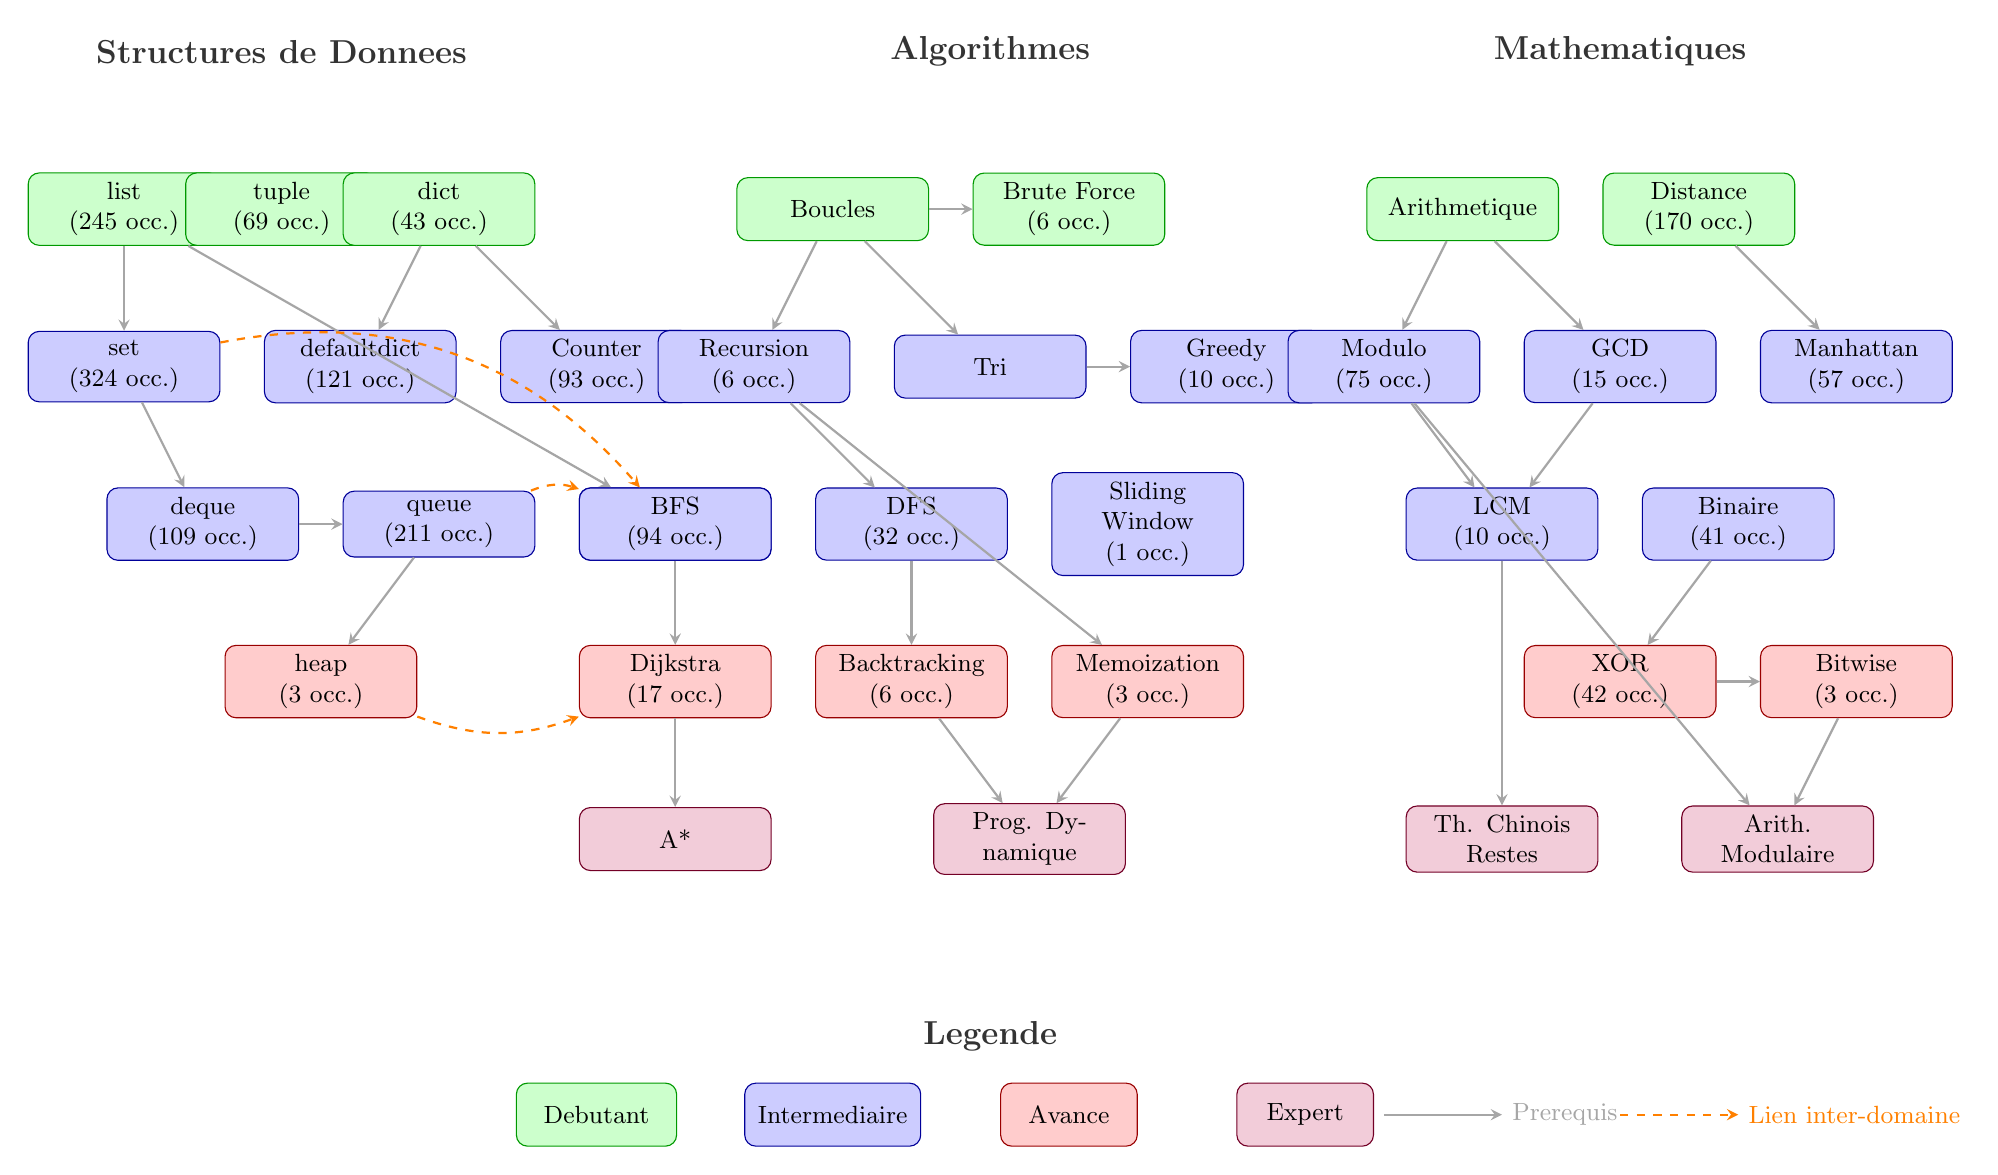
\begin{tikzpicture}[
    % Styles des noeuds par niveau
    debutant/.style={rectangle, rounded corners, draw=green!60!black, fill=green!20,
                     text width=2.2cm, align=center, minimum height=0.8cm, font=\small},
    intermediaire/.style={rectangle, rounded corners, draw=blue!60!black, fill=blue!20,
                          text width=2.2cm, align=center, minimum height=0.8cm, font=\small},
    avance/.style={rectangle, rounded corners, draw=red!60!black, fill=red!20,
                   text width=2.2cm, align=center, minimum height=0.8cm, font=\small},
    expert/.style={rectangle, rounded corners, draw=purple!60!black, fill=purple!20,
                   text width=2.2cm, align=center, minimum height=0.8cm, font=\small},
    % Style des fleches
    arrow/.style={->, >=stealth, thick, color=gray!70},
    % Style des labels de section
    section/.style={font=\bfseries\large, color=black!80}
]

% ==========================================
% SECTION 1: STRUCTURES DE DONNEES (gauche)
% ==========================================
\node[section] at (-6, 8) {Structures de Donnees};

% Niveau Debutant
\node[debutant] (list) at (-8, 6) {list\\(245 occ.)};
\node[debutant] (tuple) at (-6, 6) {tuple\\(69 occ.)};
\node[debutant] (dict) at (-4, 6) {dict\\(43 occ.)};

% Niveau Intermediaire
\node[intermediaire] (set) at (-8, 4) {set\\(324 occ.)};
\node[intermediaire] (defaultdict) at (-5, 4) {defaultdict\\(121 occ.)};
\node[intermediaire] (counter) at (-2, 4) {Counter\\(93 occ.)};

% Niveau Intermediaire+
\node[intermediaire] (deque) at (-7, 2) {deque\\(109 occ.)};
\node[intermediaire] (queue) at (-4, 2) {queue\\(211 occ.)};
\node[intermediaire] (stack) at (-1, 2) {stack\\(98 occ.)};

% Niveau Avance
\node[avance] (heap) at (-5.5, 0) {heap\\(3 occ.)};

% Fleches structures
\draw[arrow] (list) -- (set);
\draw[arrow] (dict) -- (defaultdict);
\draw[arrow] (dict) -- (counter);
\draw[arrow] (set) -- (deque);
\draw[arrow] (deque) -- (queue);
\draw[arrow] (list) -- (stack);
\draw[arrow] (queue) -- (heap);

% ==========================================
% SECTION 2: ALGORITHMES (centre)
% ==========================================
\node[section] at (3, 8) {Algorithmes};

% Niveau Debutant
\node[debutant] (boucles) at (1, 6) {Boucles};
\node[debutant] (brute) at (4, 6) {Brute Force\\(6 occ.)};

% Niveau Intermediaire
\node[intermediaire] (recursion) at (0, 4) {Recursion\\(6 occ.)};
\node[intermediaire] (tri) at (3, 4) {Tri};
\node[intermediaire] (greedy) at (6, 4) {Greedy\\(10 occ.)};

% Niveau Intermediaire+
\node[intermediaire] (bfs) at (-1, 2) {BFS\\(94 occ.)};
\node[intermediaire] (dfs) at (2, 2) {DFS\\(32 occ.)};
\node[intermediaire] (sliding) at (5, 2) {Sliding Window\\(1 occ.)};

% Niveau Avance
\node[avance] (dijkstra) at (-1, 0) {Dijkstra\\(17 occ.)};
\node[avance] (backtrack) at (2, 0) {Backtracking\\(6 occ.)};
\node[avance] (memo) at (5, 0) {Memoization\\(3 occ.)};

% Niveau Expert
\node[expert] (astar) at (-1, -2) {A*};
\node[expert] (dp) at (3.5, -2) {Prog. Dynamique};

% Fleches algorithmes
\draw[arrow] (boucles) -- (brute);
\draw[arrow] (boucles) -- (recursion);
\draw[arrow] (boucles) -- (tri);
\draw[arrow] (tri) -- (greedy);
\draw[arrow] (recursion) -- (dfs);
\draw[arrow] (recursion) -- (memo);
\draw[arrow] (dfs) -- (backtrack);
\draw[arrow] (memo) -- (dp);
\draw[arrow] (backtrack) -- (dp);

% Connexions inter-sections
\draw[arrow, dashed, color=orange] (queue) to[bend left=20] (bfs);
\draw[arrow, dashed, color=orange] (set) to[bend left=30] (bfs);
\draw[arrow] (bfs) -- (dijkstra);
\draw[arrow, dashed, color=orange] (heap) to[bend right=20] (dijkstra);
\draw[arrow] (dijkstra) -- (astar);

% ==========================================
% SECTION 3: MATHEMATIQUES (droite)
% ==========================================
\node[section] at (11, 8) {Mathematiques};

% Niveau Debutant
\node[debutant] (arith) at (9, 6) {Arithmetique};
\node[debutant] (distance) at (12, 6) {Distance\\(170 occ.)};

% Niveau Intermediaire
\node[intermediaire] (modulo) at (8, 4) {Modulo\\(75 occ.)};
\node[intermediaire] (gcd) at (11, 4) {GCD\\(15 occ.)};
\node[intermediaire] (manhattan) at (14, 4) {Manhattan\\(57 occ.)};

% Niveau Intermediaire+
\node[intermediaire] (lcm) at (9.5, 2) {LCM\\(10 occ.)};
\node[intermediaire] (binary) at (12.5, 2) {Binaire\\(41 occ.)};

% Niveau Avance
\node[avance] (xor) at (11, 0) {XOR\\(42 occ.)};
\node[avance] (bitwise) at (14, 0) {Bitwise\\(3 occ.)};

% Niveau Expert
\node[expert] (crt) at (9.5, -2) {Th. Chinois\\Restes};
\node[expert] (modular) at (13, -2) {Arith.\\Modulaire};

% Fleches maths
\draw[arrow] (arith) -- (modulo);
\draw[arrow] (arith) -- (gcd);
\draw[arrow] (distance) -- (manhattan);
\draw[arrow] (gcd) -- (lcm);
\draw[arrow] (modulo) -- (lcm);
\draw[arrow] (binary) -- (xor);
\draw[arrow] (xor) -- (bitwise);
\draw[arrow] (lcm) -- (crt);
\draw[arrow] (modulo) -- (modular);
\draw[arrow] (bitwise) -- (modular);

% ==========================================
% LEGENDE
% ==========================================
\node[section] at (3, -4.5) {Legende};
\node[debutant, text width=1.8cm] at (-2, -5.5) {Debutant};
\node[intermediaire, text width=2cm] at (1, -5.5) {Intermediaire};
\node[avance, text width=1.5cm] at (4, -5.5) {Avance};
\node[expert, text width=1.5cm] at (7, -5.5) {Expert};

\draw[arrow] (8, -5.5) -- (9.5, -5.5) node[right, font=\small] {Prerequis};
\draw[arrow, dashed, color=orange] (11, -5.5) -- (12.5, -5.5) node[right, font=\small] {Lien inter-domaine};

\end{tikzpicture}
